\documentclass[12pt,a4paper]{article}
\usepackage[a4paper, left=3.5cm, right=2cm, top=2.5cm, bottom=3cm,footskip=.25in]{geometry}
\usepackage[utf8]{inputenc}
\usepackage[T1]{fontenc}
\usepackage{amsmath}
\usepackage{amssymb}
\usepackage{lmodern}
\usepackage{indentfirst}
\usepackage{enumerate}
\usepackage{array}
\usepackage{float}
\usepackage{ragged2e}
\usepackage{lipsum}
\usepackage{titlesec}
\usepackage[pdftex]{graphicx}
\graphicspath{{.png}{images/}}
\renewcommand{\baselinestretch}{1.8}

\usepackage{algorithm}
\usepackage{algpseudocode}
\usepackage{setspace}
\usepackage[table]{xcolor}
\usepackage{booktabs}

\usepackage{pdfpages}

\usepackage{hyperref}
\hypersetup{colorlinks=true, linkcolor=black}

\titlespacing*{\section}
{0pt}{5.5ex plus 1ex minus .2ex}{4.3ex plus .2ex}
\titlespacing*{\subsection}
{0pt}{5.5ex plus 1ex minus .2ex}{4.3ex plus .2ex}

\usepackage{soul}
\newcommand{\ol}[1]{{\setul{-1.2em}{}\ul{#1}}}
\newcommand{\textoverline}[1]{{\setul{-5em}{}$\overline{\mbox{#1}}$}}

\newtheorem{definition}{Definition}[subsection]
\newtheorem{example}{Example}[subsection]

\usepackage[round]{natbib}
\usepackage{tikz-qtree}
\usepackage{tikz}
\usetikzlibrary{arrows}
\usetikzlibrary{decorations.text}

\usepackage{pifont}
\newcommand{\xmark}{\ding{53}}

\begin{document}

\begin{titlepage}
	\centering
	\par\vspace{1cm}
	{\scshape\bf FACULTY OF MATHEMATICS, PHYSICS AND INFORMATICS \par}
	{\scshape\bf OF THE COMENIUS UNIVERSITY IN BRATISLAVA \par}
	\par\vspace{8cm}
	{\scshape\bf OPTIMIZATION OF AN ABDUCTIVE REASONER FOR DESCRIPTION LOGICS \par}
	\par\vspace{0.5cm}
	{\textsc Master thesis \par}
	\par\vspace{10.6cm}
	{\scshape\bf 2019 \hfill Katarína Fabianová \par}
\end{titlepage}

\pagebreak
\thispagestyle{empty}
\centering
\par\vspace{1cm}
{\scshape\bf FACULTY OF MATHEMATICS, PHYSICS AND INFORMATICS \par}
{\scshape\bf OF THE COMENIUS UNIVERSITY IN BRATISLAVA \par}
\par\vspace{8cm}
{\scshape\bf OPTIMIZATION OF AN ABDUCTIVE REASONER FOR DESCRIPTION LOGICS \par}
\par\vspace{0.5cm}
{\textsc Master thesis \par}
\par\vspace{2cm}
\begin{table*}[ht]
	\newcolumntype{x}[1]{>{\hspace{0pt}}p{#1}}
	\begin{tabular}{@{}x{5cm}x{10cm}@{}}
		Study program: & Applied informatics \\
		Field of study: & 2511 Applied informatics \\
		School department: & Department of Applied Informatics \\
		Adviser: & Mgr. Júlia Pukancová, PhD. \\
		Consultant: & RNDr. Martin Homola, PhD. \\
	\end{tabular}
\end{table*}
\par\vspace{3.03cm}
{\scshape\bf Bratislava 2019 \hfill Katarína Fabianová \par}

\pagebreak

\justify

%\pagebreak
%\thispagestyle{empty}
%\par\vspace*{15cm}
%{\large\bf Dedication \par}
%\par\vspace{0.8cm}
%\large Čestne prehlasujem, že prácu som vypracovala samostatne
%pod vedením školiteľa a uviedla som všetky použité
%zdroje informácií a použitú literatúru. \par
%\par\vspace{3cm}
%\large {Bratislava \hfill \textoverline{Katarína Fabianová}} \par

\pagebreak
\thispagestyle{empty}
\par\vspace*{15cm}
{\large\bf Acknowledgements \newline \par}

\pagebreak
\thispagestyle{empty}
{\large\bf Abstract \newline \par} 

\textbf{Key words:}

\pagebreak
\thispagestyle{empty}
{\large\bf Abstrakt \newline \par} 

\textbf{Kľúčové slová:}

\pagebreak
\thispagestyle{empty}
\tableofcontents
\thispagestyle{empty}

\pagebreak
\thispagestyle{empty}
\listoffigures

\pagebreak
\setcounter{page}{1}
\section*{Introduction}
\addcontentsline{toc}{section}{\protect\numberline{}Introduction}


\pagebreak
\section{Description logics}
Description logics (DLs) are a family of knowledge representation formalism. Each description logic has different expressivity. Every expressivity is expressed with a unique set of constructors. We are going to work with $\mathcal{ALC}$, $\mathcal{EL}$ and $\mathcal{EL}${+}{+} DL. Each description logic has its own syntax and semantics. In this chapter we will introduce syntax and semantics \citep{Rudolph2011} for each DL that we will be working with.

\subsection{$\mathcal{ALC}$ DL}
$\mathcal{ALC}$ DL is a DL which is more expressive than $\mathcal{EL}$ and $\mathcal{EL}{+}{+}$ DL. $\mathcal{ALC}$ is less expressive than many other DLs. $\mathcal{ALC}$ stands for Attributive (Concept) Language with Complements. It means that not only complement of atomic concept is allowed but also a complement of complex concept is allowed.

\subsubsection{$\mathcal{ALC}$ Syntax}
$\mathcal{ALC}$ description logic consists of three mutually disjoint sets. These sets (definition~\ref{def:DLVocabulary}) represent whole vocabulary that is used by $\mathcal{ALC}$ DL.

\begin{definition}{\textbf{DL vocabulary}}
	\label{def:DLVocabulary}
	
	\[ \textbf{Set of individuals:} \text{ } N_{I} = \{a,b,c...\} \]
	\[ \textbf{Set of concepts:} \text{ } N_{C} = \{A,B,C...\} \]
	\[ \textbf{Set of roles:} \text{ } N_{R} = \{R_{1},R_{2},R_{3},...\} \]
\end{definition}

\begin{example}{\textbf{DL vocabulary}}
	\[ N_{I} = \{ jack, john, jane \} \]
	\[ N_{C} = \{ Person, Mother, Father \} \]
	\[ N_{R} = \{ hasChild, likes, owns \} \]
\end{example}

$\mathcal{ALC}$ DL deals with individuals and concepts. An individual is a concrete instance of a concept. Concept is a class that defines some entity. Concept can be atomic or complex. Atomic concept is not constructed with any constructor. On the contrary complex concept is created from constructors and other concepts.

\begin{definition}{\textbf{Complex concept}}
	\label{def:complexConcept}
	
	Concepts are recursively constructed as the smallest set of expressions of the forms:
	\[ C,D ::= A | \neg C | C \sqcap D | C \sqcup D | \exists R.C | \forall R.C \]
	where $A \in N_{C}$, $R \in N_{R}$, and C, D are concepts.
\end{definition}

Practical usage of definition ~\ref{def:complexConcept} is shown in example~\ref{example:complexConcept}.

\begin{example}{\textbf{Complex concept}}
	\label{example:complexConcept}
\[ \neg Mother \]
\[ Mother \sqcup Father \]
\[ \exists hasChild.Person \]
\[ \forall likes.Food \]
\end{example}

Complex concept uses following constructors: $\neg$, $\sqcup$, $\sqcap$, $\exists$ and $\forall$. Constructor $\neg$ is negation, constructor $\sqcup$ is or and constructor $\sqcap$ is and. Constructors $\exists$ is existential restriction and $\forall$ is called value restriction.

There are two concepts that are always in ontology. $\top$ (top) stays for everything. Each concept belongs under $\top$ which means that each concept is on left side of subsumption if on right side is only $\top$. Second concept is $\bot$ (bottom) and it stays for nothing which means that each concept is on the right side of subsumption if there is only $\bot$ on the left side. Formally these two concepts can be written as we see in definition~\ref{def:topBottom}.

\begin{definition}{\textbf{Top and Bottom}}
	\label{def:topBottom}
	\[ \top \equiv A \sqcup \neg A \] 
	\[ \bot \equiv A \sqcap \neg A \]
\end{definition}

$\mathcal{ALC}$ description logic uses axioms in order to model some situation. Ontology \citep{staabHandbookOntology} is used to formally describe these axioms. The purpose of ontology is to describe relationships between entities in a formal language. Every ontology has its own knowledge base. Knowledge base is a set of TBox axioms and ABox axioms. Ontology is described by knowledge base. Knowledge base is defined in definition~\ref{def:knowledgeBase}.

\begin{definition}{\textbf{Knowledge base}}
	\label{def:knowledgeBase}
	
	Knowledge base ($\mathcal{KB}$) is an ordered pair of \textit{TBox} $\mathcal{T}$ and \textit{ABox} $\mathcal{A}$.
\end{definition}

An example for knowledge base is shown in example ~\ref{example:knowledgeBase}.

\begin{example}{\textbf{Knowledge base}}
	\label{example:knowledgeBase}
	\[ 
	\mathcal{KB} = \left\{
	\begin{tabular}{c c}
	$Professor \sqcup Scientist \sqsubseteq Academician$ \\
	$AssocProfessor \sqsubseteq Professor$ \\
	$jack : Academician$ \\
	$jane : Scientist$ \\
	$john : Professor$ \\	
	\end{tabular}
	\right \}
	\]
\end{example}

There are two types of axioms, the first is TBox (definition~\ref{def:tbox}) and the second one is ABox (definition~\ref{def:abox}). In TBox the subsumption symbol ($\sqsubseteq$) is used. Let's explain this symbol on an example $Mother \sqsubseteq Parent$. $Mother$ is always a $Parent$ but $Parent$ does not always have to be a $Mother$. TBox represents axioms that model ontology. Each axiom explains the relationship between entities in this axiom.

\begin{definition}{\textbf{TBox}}
	\label{def:tbox}
	
	A TBox $\mathcal{T}$ is a finite set of GCI axioms $\phi$ of the form:
	\[ \phi ::= C \sqsubseteq D \]	
	where C, D are any concepts.
\end{definition}

\begin{example}{\textbf{TBox}}
	\[ 
	\mathcal{T} = \left\{
	\begin{tabular}{c c}
	$Professor \sqcup Scientist \sqsubseteq Academician$ \\
	$AssocProfessor \sqsubseteq Professor$ \\
	\end{tabular}
	\right \}
	\]
\end{example}

ABox on the other side does not model ontology but creates a database of facts. It contains set of assertion axioms that can be called facts. Fact is a direct assertion of an individual to a concept.

\newpage
\begin{definition}{\textbf{ABox}}
	\label{def:abox}
	
    An ABox $\mathcal{A}$ is a finite set of assertion axioms $\phi$ of the form:
	\[ \phi ::= a:C | a,b:R \]
	where $a,b \in N_{I}$, $R \in N_{R}$ and C is any concept.
\end{definition}

\begin{example}{\textbf{ABox}}
	\[ 
	\mathcal{A} = \left\{
	\begin{tabular}{c c}
	$jack : Academician$ \\
	$jane : Scientist$ \\
	$john : Professor$ \\
	\end{tabular}
	\right \}
	\]
\end{example}

To have a better understanding of $\mathcal{ALC}$ DL we can translate sentences into $\mathcal{ALC}$ description logic (example~\ref{example:sentences}).

\begin{example}{\textbf{ABox}}
	\label{example:sentences}
	
	\begin{table}[H]
		\centering
		\begin{tabular}{c c}
			Everybody who is sick, is not happy & $Sick \sqsubseteq \neg Happy$ \\ \addlinespace[0.5cm]
			Cat and dogs are animals. & $Cat \sqcup Dog \sqsubseteq Animal$ \\ \addlinespace[0.5cm]
			Every person owns a house. & $Person \sqsubseteq \exists owns.House$ \\	\addlinespace[0.5cm]
		\end{tabular}		
	\end{table}
\end{example}

\subsubsection{$\mathcal{ALC}$ Semantics}
An interpretation is a pair of a domain and an interpretation function. The domain is a set of values that represents concepts in the interpretation (definition~\ref{def:interpretation}). The result of interpretation function is different for individuals, concepts and roles. If we use the interpretation function on an individual the result is an element from the domain. If we use it on the concepts the result is a set of elements from the domain. If we use it on the roles the result is a set of pairs of elements from the domain.

\newpage
\begin{definition}{\textbf{Interpretation}}
	\label{def:interpretation}

	An interpretation of a given knowledge base $\mathcal{KB} = (\mathcal{T}, \mathcal{A})$ is a pair $\mathcal{I} = (\Delta^{\mathcal{I}}, \cdot ^{\mathcal{I}})$ which contains a domain $\Delta^{\mathcal{I}}$ and an interpretation function $\cdot ^{\mathcal{I}}$.	
	Domain can not be empty.
		
	The interpretation function is following:
	\[ a^{\mathcal{I}} \in \Delta^{\mathcal{I}} \text{ } \forall a \in N_{I} \]
	\[ A^{\mathcal{I}} \subseteq \Delta^{\mathcal{I}} \text{ } \forall A \in N_{C} \]
	\[ R^{\mathcal{I}} \subseteq \Delta^{\mathcal{I}} \times \Delta^{\mathcal{I}} \text{ } \forall R \in N_{R} \]
	The interpretation of complex concepts is recursively defined:
	\[ \neg C^{\mathcal{I}} = \Delta^{\mathcal{I}} \backslash C^{\mathcal{I}} \]
	\[ C \sqcap D^{\mathcal{I}} = C^{\mathcal{I}} \cap D^{\mathcal{I}} \]
	\[ C \sqcup D^{\mathcal{I}} = C^{\mathcal{I}} \cup D^{\mathcal{I}} \]
	\[ \exists R.C^{\mathcal{I}} = \{ x \in \Delta^{\mathcal{I}} | \exists y \in \Delta^{\mathcal{I}} : \langle x,y \rangle \in R^{\mathcal{I}} \land y \in C^{\mathcal{I}} \} \]
	\[ \forall R.C^{\mathcal{I}} = \{ x \in \Delta^{\mathcal{I}} | \forall y \in \Delta^{\mathcal{I}} : \langle x,y \rangle \in R^{\mathcal{I}} \rightarrow y \in C^{\mathcal{I}} \} \]
\end{definition}

\newpage
\begin{example}{\textbf{Interpretation}}
	\[ 
	\mathcal{KB} = \left\{
	\begin{tabular}{c c}
	$Professor \sqcup Scientist \sqsubseteq Academician$ \\
	$AssocProfessor \sqsubseteq Professor$ \\
	$jack : Academician$ \\
	\end{tabular}
	\right \}
	\]
	
	\[ \mathcal{I} = (\Delta ^{\mathcal{I}}, \cdot^{\mathcal{I}}) \]
	\[ \Delta ^{\mathcal{I}} = \{ P,S,A,AP \} \]
	\[ Professor^{\mathcal{I}} = \{P\} \]
	\[ Scientist^{\mathcal{I}} = \{S\} \]
	\[ Academician^{\mathcal{I}} = \{A\} \]
	\[ AssocProfessor^{\mathcal{I}} = \{AP\} \]
	\[ jack^{\mathcal{I}} = A \]
	
\end{example}

The interpretation satisfies (definition~\ref{def:satisfaction}) an axiom according to its type. We know three types of axioms. The first is an axiom from TBox, the second one is an assertion axiom to a concept and the third one is an assertion to a role.

\begin{definition}{\textbf{Satisfaction $\models$}}
	\label{def:satisfaction}

	Given an axiom $\phi$, an interpretation $\mathcal{I} = (\Delta^{\mathcal{I}}, \cdot ^{\mathcal{I}})$ satisfies $\phi (\mathcal{I} \models \phi)$ depending on its type:
	\[ \mathcal{I} \models C \sqsubseteq D \text{ iff } C^{\mathcal{I}} \subseteq D^{\mathcal{I}} \]
	\[ \mathcal{I} \models a:C \text{ iff } a^{\mathcal{I}} \in C^{\mathcal{I}} \]
	\[ \mathcal{I} \models a,b:R \text{ iff } \langle a^{\mathcal{I}}, \in b^{\mathcal{I}} \rangle \in R^{\mathcal{I}} \]	
\end{definition}

Finding a model (an interpretation satisfying $\mathcal{KB}$, definition~\ref{def:model}) is crucial for consistency checking. If we find at least one model the knowledge base $\mathcal{KB}$ is consistent. We can have more models for one knowledge base. In example~\ref{example:model} there are two showed models but there can be more models. 

\begin{definition}{\textbf{Model}}
	\label{def:model}

	An interpretation $\mathcal{I} = \langle \Delta^{\mathcal{I}}, \cdot ^{\mathcal{I}}  \rangle$ is a model of a DL knowledge base $\mathcal{KB} = (\mathcal{T}, \mathcal{A})$ iff $\mathcal{I}$ satisfies every axiom in TBox $\mathcal{T}$ and ABox $\mathcal{A}$.
\end{definition}

\begin{example}{\textbf{Model}}
	\label{example:model}
	\[ 
	\mathcal{KB} = \left\{
	\begin{tabular}{c c}
	$Professor \sqcup Scientist \sqsubseteq Academician$ \\
	$AssocProfessor \sqsubseteq Professor$ \\
	$jack : Academician$ \\
	\end{tabular}
	\right \}
	\]

	\[ \mathcal{I}_{1} = \{  \Delta^{\mathcal{I}} = \{ P,S,A,AP \}, \]	
	\[ Professor^{\mathcal{I}} = \{P\}, Scientist^{\mathcal{I}} = \{S\}, Academician^{\mathcal{I}} = \{A\}, AssocProfessor^{\mathcal{I}} = \{AP\} \]
	\[ jack^{\mathcal{I}} = A \} \]	

	\[ \mathcal{I}_{2} = \{  \Delta^{\mathcal{I}} = \{ A \}, \]	
	\[ Professor^{\mathcal{I}} = \{A\}, Scientist^{\mathcal{I}} = \{A\}, Academician^{\mathcal{I}} = \{A\}, AssocProfessor^{\mathcal{I}} = \{A\} \]
	\[ jack^{\mathcal{I}} = A \} \]		
\end{example}

\begin{definition}{\textbf{Consistency}}
	
	A knowledge base $\mathcal{KB}$ is consistent iff $\mathcal{KB}$ has at least one model $\mathcal{I}$.
\end{definition}

We are familiar with more decision problems, satisfiability, subsumption $(\sqsubseteq)$, equivalence ($\equiv$) and disjointness. Satisfiability means that concept is satisfiable in regard to $\mathcal{KB}$ if we can find such a model of a knowledge base for which holds that interpretation of that concept is not empty. Subsumption between two concepts must hold that interpretation of left-sided concept is a proper subset of interpretation of right-sided concept in each possible model of a knowledge base. Equivalence is similar to subsumption but the difference is that the interpretations of both concepts must be equal in each possible model of a knowledge base. Disjointness means that intersection of the interpretations of both concepts must be an empty set in each possible model of a knowledge base.

\begin{definition}{\textbf{Decision problems}}

	Given a DL $\mathcal{KB} = (\mathcal{T}, \mathcal{A})$, and two concepts C,D, we say that:

	\begin{itemize}
		\item $C \text{ is satisfiable w.r.t. } \mathcal{KB} \text{ iff there is such a model } \mathcal{I} \text{ of } \mathcal{KB} \text{ for which holds that } \newline C^{\mathcal{I}} \neq \emptyset;$

		\item $C \text{ is subsumed by D w.r.t. } \mathcal{KB} \text{ (denoted } \mathcal{KB} \models C \sqsubseteq D) \text{ iff } C^{\mathcal{I}} \subseteq D^{\mathcal{I}} \text{ in every} \newline \text{model } \mathcal{I} \text{ of } \mathcal{KB};$

		\item $\text{C and D are equivalent w.r.t. } \mathcal{KB} \text{ (denoted } \mathcal{KB} \models C \equiv D) \text{ iff } C^{\mathcal{I}} = D^{\mathcal{I}} \text{ in every} \newline \text{model } \mathcal{I} \text{ of } \mathcal{KB};$
		
		\item $\text{C and D are disjoint w.r.t. } \mathcal{KB} \text{ iff } C^{\mathcal{I}} \cap D^{\mathcal{I}} = \emptyset \text{ in every model } \mathcal{I} \text{ of } \mathcal{KB}.$		
	\end{itemize}
\end{definition}

If $\mathcal{KB} = \emptyset$ then we say that decision problems (satisfiability, subsumption, equivalence and disjointness) of concepts are defined in general by definition and we use notation such as we omit $\mathcal{KB} \models$ from the notation.

\subsection{DL Tableau algorithm}
Following definitions \citep{baaderHandbook} describe rules and terms that are used by this algorithm. DL Tableau algorithm proves satisfiability of a concept or checks consistency of a given knowledge base. By proving satisfiability the input for the algorithm is concept C and TBox $\mathcal{T}$. By checking consistency the input for the algorithm is a knowledge base $\mathcal{KB}$. In both versions of this algorithm holds that each concept must be in NNF (negation normal form, definition ~\ref{def:nnf}). Negation normal form is such a form that each negation is pushed in front of atomic concept inside a complex concept. 

\begin{definition}{\textbf{NNF}}
	\label{def:nnf}
	
	A concept C is in NNF (negation normal form) iff the complement constructor $\neg$ 
	only occurs in front of atomic concept symbols inside C.
\end{definition}

\begin{example}{\textbf{NNF}}
	\[ nnf(\neg (C \sqcap D)) = \neg C \sqcup \neg D \]
	\[ nnf(\neg (C \sqcup D)) = \neg C \sqcap \neg D \]
	\[ nnf(\neg \exists R.C) = \forall R. \neg C \]
	\[ nnf(\neg \forall R.C) = \exists R. \neg C \]
\end{example}

DL Tableau algorithm creates a CTree (Completion tree, definition~\ref{def:ctree}). CTree proves whether model exists or not.

\begin{definition}{\textbf{Completion tree}}
	\label{def:ctree}

	A completion tree (CTree) is a triple T = (V, E, $\mathcal{L}$) where (V, E)
	is a tree and $\mathcal{L}$ is a labeling function which means that:
	$\mathcal{L}(x)$ is a set of concepts $\forall x \in V$ and
	$\mathcal{L}(\langle x, y \rangle )$ is a set of roles $\forall \langle x, y \rangle \in E$.	
\end{definition}

At first the algorithm creates node and initializes it with the input concept.
Then the algorithm applies tableau rules for given DL. If the algorithm applies each rule until any rule can be applied and it finds no clash then result is that concept C is satisfiable w.r.t. $\mathcal{T}$. Children of a node are called successors or R-successors (definition~\ref{def:successor}).

\begin{definition}{\textbf{Successor, R-successor}}
	\label{def:successor}

	Given a CTree T = (V,E, $\mathcal{L}$) and $x,y \in V$ we say that: 
	\begin{itemize}
		\item y is a successor of x iff $\langle x,y \rangle \in E$
		\item y is an R-successor of x iff $\langle x,y \rangle \in E$ and $R \in \mathcal{L}(\langle x,y \rangle)$.
	\end{itemize}
\end{definition}

A clash containing Ctree is such a tree that one branch of this tree contains a concept and simultaneously its negation too. Clash is defined in definition~\ref{def:clash}.

\begin{definition}{\textbf{Clash}}
	\label{def:clash}

	There is a clash in a CTree T = $(V,E, \mathcal{L})$ if and only iff for some $x \in V$ and for some concept C both $C \in \mathcal{L}(x)$ and $\neg C \in \mathcal{L}(x)$.
\end{definition}

\begin{example}{\textbf{Clash}}
	\[ \mathcal{L}(s_{0}) = \{ C, D, \neg D \} \]
\end{example}

\begin{definition}{\textbf{Clash-free CTree}}

A CTree T = $(V,E, \mathcal{L})$ is clash-free iff none of the nodes in V contains a clash.
\end{definition}

There can be a situation that some concept can lead to infinite looping and algorithm would never stop. This situation is called blocking (definition~\ref{def:blocking}). An example for that is: $Person \sqsubseteq \exists hasParent.Person$. That is why the algorithm uses Blocking rule.

\begin{definition}{\textbf{Blocking}}
	\label{def:blocking}
	
	Given a CTree $T = (V, E, \mathcal{L})$ a node $x \in V$ is blocked if it has an ancestor $y$ such that: either $\mathcal{L}(x) \subseteq \mathcal{L}(y)$ or $y$ is blocked.
\end{definition}

DL Tableau algorithm proves concept satisfiability in regard of TBox (definition~\ref{def:conceptSatisfiability}). Input for DL Tableau algorithm is concept C and TBox $\mathcal{T}$. Output is a boolean value which is true if concept C is satisfiable w.r.t. $\mathcal{T}$, false otherwise.

\begin{definition}{\textbf{Algorithm -- Concept satisfiability}}	
	\label{def:conceptSatisfiability}

	\textbf{Input:} concept C and $\mathcal{T}$ in NNF \newline
	\indent \textbf{Output:} answers whether concept C is satisfiable w.r.t. $\mathcal{T}$ or not \newline
	\indent \textbf{Steps:}
	\begin{enumerate}
		\item Initialize a new CTree T := $(\{s_{0}\}, \emptyset, \{s_{0} \rightarrow \{C\}\})$;
		\item Apply tableau rules for TBoxes while at least one rule is applicable;
		\item Answer "C is satisfiable w.r.t. $\mathcal{T}$" if T is clash-free. Otherwise answer "C is unsatisfiable w.r.t. $\mathcal{T}$".
	\end{enumerate}
\end{definition}

\begin{definition}{\textbf{$\mathcal{ALC}$ tableau rules for TBoxes}}
	\begin{itemize}
		\item $\sqcap-rule:$ if $C_{1} \sqcap C_{2} \in \mathcal{L}(x)$ and $x \in V$ and $\{ C_{1}, C_{2} \} \not \subseteq \mathcal{L}(x)$ and x is not blocked then $\mathcal{L}(x) = \mathcal{L}(x) \cup \{ C_{1}, C_{2} \}$
		
		\item $\sqcup-rule:$ if $C_{1} \sqcup C_{2} \in \mathcal{L}(x)$ and $x \in V$ and $ \{ C_{1}, C_{2} \} \cap \mathcal{L}(x) = \emptyset$ and x is not blocked then either $\mathcal{L}(x) = \mathcal{L}(x) \cup \{ C_{1} \}$ or $\mathcal{L}(x) = \mathcal{L}(x) \cup \{ C_{2} \}$
		
		\item $\forall-rule:$ if $\forall R.C \in \mathcal{L}(x)$ and $x,y \in V$ and y is R-successor of x and $C \not \in \mathcal{L}(y)$ and x is not blocked then $\mathcal{L}(y) = \mathcal{L}(y) \cup \{ C \}$
		
		\item $\exists-rule:$ if $\exists R.C \in \mathcal{L}(x)$ and $x \in V$ with no R-successor y and $C \in \mathcal{L}(y)$ and x is not blocked then $\mathcal{V} = \mathcal{V} \cup \{ z \}, \mathcal{L}(z) = \{ C\}$ and $\mathcal{L}( \langle x, z \rangle ) = \{ R \}$
		
		\item $\mathcal{T}-rule:$ if $C_{1} \sqsubseteq C_{2} \in \mathcal{T}$ and $x \in V$ and nnf$(\neg C_{1} \sqcup C_{2}) \not \in \mathcal{L}(x)$ and x is not blocked then $\mathcal{L}(x) = \mathcal{L}(x) \cup \{ nnf(\neg C_{1} \sqcup C_{2}) \}$
	\end{itemize}
\end{definition}	

Knowledge base is a pair of a TBox and an Abox and yet only a TBox was mentioned in connection with the DL Tableau algorithm. If we also have a given ABox the algorithm must be modified. The algorithm checks no longer concept satisfiability w.r.t. $\mathcal{T}$ but checks consistency of a given $\mathcal{KB}$. The same condition holds for the result as in proving concept satisfiability. If there is a found clash the knowledge base is not consistent otherwise the knowledge base is consistent (definition~\ref{def:consistency}). Difference between the first version of this algorithm is that here are used named nodes. Name of the node is an instance of a concept that comes from ABox. 

\begin{definition}{\textbf{Algorithm -- Consistency checking}}
	\label{def:consistency}

\textbf{Input:} $\mathcal{KB} = (\mathcal{T}, \mathcal{A})$ in NNF \newline
\indent \textbf{Output:} answers whether $\mathcal{KB}$ is consistent or not \newline
\indent \textbf{Steps:}
\begin{enumerate}
	\item Initialize a CTree as follows:
		\begin{itemize}
			\item $V := \{ a \text{ } | \text{ individual a occurs in } \mathcal{A} \}$;
			\item $E := \{ \langle a,b \rangle \text{ } | \text{ } a,b : R \in \mathcal{A} \text{ for some role R} \}$;
			\item $\mathcal{L}(a) := \{ nnf(E) \text{ } | \text{ } a:E \in \mathcal{A}\} \text{ for all } a \in V$; \newline
			$\mathcal{L}(\langle a,b \rangle) := \{ R \text{ } | \text{ } a,b:R \in \mathcal{A}\} \text{ for all } \langle a,b \rangle \in E$;
		\end{itemize}
	\item Apply tableau rules for TBoxes while at least one rule is applicable;
	\item Answer "$\mathcal{KB}$ is consistent" if T is clash-free. Otherwise answer "$\mathcal{KB}$ is inconsistent".
\end{enumerate}

\end{definition}

Let's introduce an example~\ref{example:dlTableau} where we know a knowledge base $\mathcal{KB}$. DL Tableau algorithm checks if knowledge base is consistent or not.

\begin{example}{(\textbf{DL Tableau algorithm})}
	\label{example:dlTableau}
	\[ 
	\mathcal{KB} = \left\{
	\begin{tabular}{c c}
	$Student \sqsubseteq \exists attends.MathCourse$ \\
	$MathCourse \sqsubseteq Course$ \\
	$jack : Student$ \\
	\end{tabular}
	\right \}
	\] \\
\end{example}

\begin{center}
	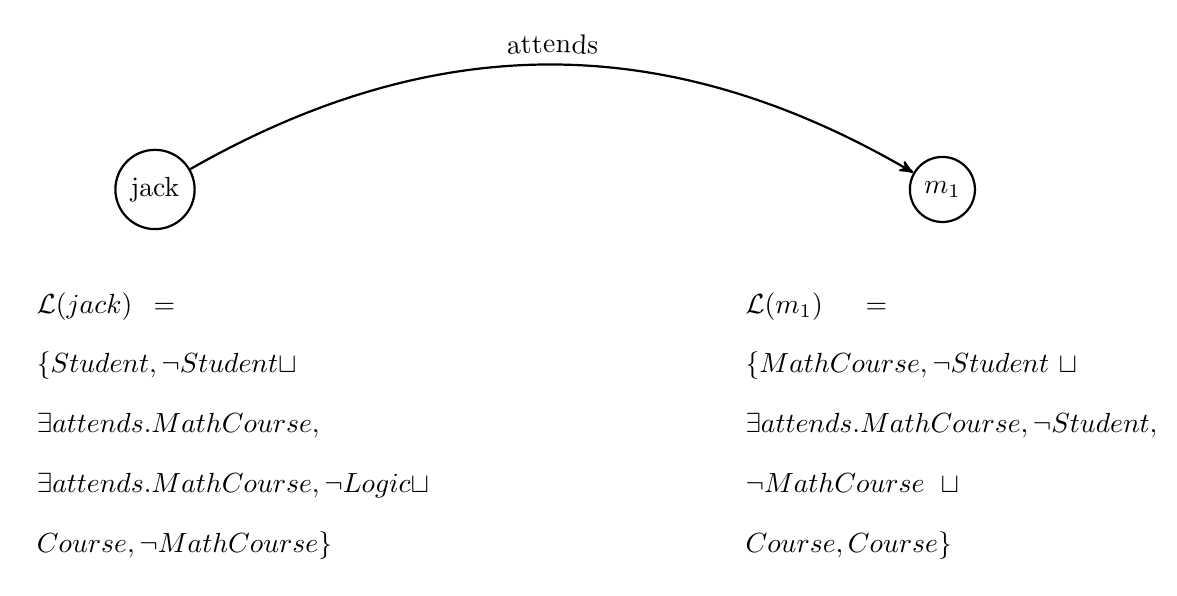
\begin{tikzpicture}[->,>=stealth',auto,node distance=10cm,
	thick,main node/.style={circle, draw}]
	
	\node[main node] (1) {jack};
	\node[main node] (2) [right of=1] {$m_{1}$};
	
	\def\myshift#1{\raisebox{1ex}}
	
	\draw [thick, ->, postaction={decorate, decoration={text along path, text align=center, text={|\myshift|attends}}}] (1) to [bend left=30] (2);
	
	\node[text width=3cm] at (0,-3) 
	{$\mathcal{L}(jack) = \{ Student, \neg Student \sqcup \exists attends.MathCourse, \newline \exists attends.MathCourse, \neg Logic \sqcup Course, \neg MathCourse \}$};		

	\node[text width=5cm] at (10,-3) 
	{$\mathcal{L}(m_{1}) = \{ MathCourse, \neg Student \sqcup \exists attends.MathCourse, \neg Student, \newline \neg MathCourse \sqcup Course, Course \}$};			
	\end{tikzpicture}
\end{center}

The algorithm starts with the ABox assertion axioms. It selects the axiom $jack : Student$. At first it creates a node $jack$ with its label $\mathcal{L}(jack)$. From the assertion axiom $jack : Student$ algorithm knows that jack is a Student and adds the concept $Student$ to the label $\mathcal{L}(jack)$. Then the algorithm is choosing another axiom from the knowledge base. There are no more assertion axioms, so it starts with the axioms from TBox. It takes $Student \sqsubseteq \exists attends.MathCourse$. It must convert it into the negation normal form which is $\neg Student \sqcup \exists attends.MathCourse$. The algorithm applies $\sqcup-rule$. According to this rule it must choose $\exists attends.MathCourse$, otherwise there would be a clash. Now it has to apply $\exists - rule$ so a new node $l_{1}$ will be created with its label $\mathcal{L}(m_{1})$. Concept $MathCourse$ will be added into this label. Let's go back to the $jack$ node. The algorithm has to finish adding all axioms of TBox form. It will add the second axiom from the knowledge base in negation normal form as $\neg MathCourse \sqcup Course$. Now it does not matter which one algorithm chooses if $Course$ or $\neg MathCourse$ because any of these two does not cause a clash. Now the algorithm goes back to the $m_{1}$ node and continues to add axioms from the knowledge base similarly as in the node $jack$. It starts with axiom $\neg Student \sqcup \exists attends.MathCourse$, it will choose the first one $\neg Student$. Then continues with axiom $\neg MathCourse \sqcup Course$. It can not choose $\neg MathCourse$ because there would be immediately a clash. So it chooses $Course$.

The created tree contains two nodes ($jack$ and $m_{1}$) and one edge between them. The edge represents that $jack$ attends some MathCourse $m_{1}$. There is not any instance of a concept $MathCourse$ so the node $m_{1}$ does not represent a concrete instance of the concept $MathCourse$ but represents some instance. There is no clash in both nodes so the answer of the DL Tableau algorithm is that the given knowledge base $\mathcal{KB}$ is consistent.

\section{Abduction}
Generally in logic we are familiar with three ways of thinking. Deduction, induction and abduction. The most known and natural for humans is probably deduction. All three ways are dealing with the following parts: theory, data and effect. In the description logic we can translate the theory as a knowledge base, data as the explanations and the effect as an observation.

By deduction a knowledge base and the explanations is known, the observation is missing and the goal is to deduce the missing observation. By induction is known an observation and an explanation but the knowledge base is unknown. By abduction is known a knowledge base and an observation but the explanation is a subject of searching. All definitions are from article by \cite{pukancovaAboxAbduction}.

\subsection{ABox abduction}
In the description logics abduction (definition~\ref{def:abduction}) is used when we are not familiar with the explanation $\mathcal{E}$ but we know a knowledge base $\mathcal{KB}$ and an observation $\mathcal{O}$. It is important to know that we are looking for minimal explanations. A minimal explanation is such an explanation that it does not exist any other explanation that would be a subset of that minimal explanation.

\begin{definition}{\textbf{(Abduction)}} 
	\label{def:abduction}
		
	Given a knowledge base $\mathcal{KB}$ and an observation $\mathcal{O}$, an abductive explanation is such an explanation $\mathcal{E}$ that satisfies $\mathcal{KB} \cup \mathcal{E} \models \mathcal{O}$.
\end{definition}

\begin{definition}{\textbf{(Correct explanation)}}
	\begin{table}[H]
		\centering
		\begin{tabular}{c}
			$\mathcal{E} \text{ is consistent if } \mathcal{E} \cup \mathcal{KB} \not \models \mathcal{\bot};$ \\
			\addlinespace[0.5cm]
			$\mathcal{E} \text{ is relevant if } \mathcal{E} \not \models \mathcal{O};$ \\
			\addlinespace[0.5cm]
			$\mathcal{E} \text{ is explanatory if } \mathcal{KB} \not \models \mathcal{O}$ \\
		\end{tabular}
	\end{table}
\end{definition}

\begin{definition}{\textbf{(Minimal explanation)}}
	
	Minimal explanation is such an explanation that it does not exist any other explanation that would be a subset of this explanation.
\end{definition}

For better understanding of what ABox abduction is let's introduce a few examples. The first example~\ref{example:abductionEmotion} is easy, the searched explanation is obvious but it will demonstrate the problem. The second example~\ref{example:abductionAcademy} is not so obvious that is why we have to use an algorithm to compute the solution. For computing the solution we use the \textbf{Minimal Hitting Set algorithm}.

\newpage
\begin{example}{(\textbf{ABox Abduction - Emotion})}
	\label{example:abductionEmotion}
	\[ 
	\mathcal{KB} = \left\{
	\begin{tabular}{c c}
	$Sick \sqsubseteq \neg Happy$
	\end{tabular}
	\right \}
	\]
	\[ 
	\mathcal{O} = \left\{
	\begin{tabular}{c c}
	$mary : \neg Happy$
	\end{tabular}
	\right \}
	\]								
\end{example}

In example~\ref{example:abductionEmotion} we are searching the explanations. In this easy assignment it is obvious that what we are looking for is that Mary is sick. If Mary is not happy she must be sick. Formally written solution to this abduction problem is the following:
\[ 
\mathcal{E} = \left\{
\begin{tabular}{c c}
$mary : Sick$
\end{tabular}
\right \}
\]

\begin{example}{(\textbf{ABox Abduction - Academy})}
	\label{example:abductionAcademy}
	\[ 
	\mathcal{KB} = \left\{
	\begin{tabular}{c c}
		$Professor \sqcup Scientist \sqsubseteq Academician$ \\
		$AssocProfessor \sqsubseteq Professor$ \\
	\end{tabular}
	\right \}
	\]
	\[ 
	\mathcal{O} = \left\{
	\begin{tabular}{c c}
		$jack : Academician$
	\end{tabular}
	\right \}
	\]								
	
\end{example}

In example~\ref{example:abductionAcademy} we search minimal explanations when we know that $jack$ is an Academician. If $jack$ is an Academician he must be a Professor or a Scientist. If he is a Professor he must be also an AssocProfessor. This is an oversimplified explanation how we can retrieve correct explanations. For the better introduction into this algorithm we will explain it step by step. We know the observation so we know that jack is an Academician, that is a fact. In our first axiom in TBox it is written that if somebody is an Academician he is also a Professor or a Scientist. He can be both but at least one of them but that we are not able to determine. That is why both explanations are correct. The second axiom claims that if somebody is a Professor he must be also an AssocProfessor. In this part we are not explaining the whole algorithm yet because it will be explained in our next chapter Minimal Hitting Set algorithm but we need to have at least an idea of how it works. So as we already know the correct explanations are following:

\[ 
\mathcal{E}_{1} = \left\{
\begin{tabular}{c c}
	$jack : Professor$ \\
\end{tabular}
\right \}
\]
\[ 
\mathcal{E}_{3} = \left\{
\begin{tabular}{c c}
	$jack : Scientist$ \\
\end{tabular}
\right \}
\]
\[ 
\mathcal{E}_{3} = \left\{
\begin{tabular}{c c}
	$jack : AssocProfessor$ \\
\end{tabular}
\right \}
\]

\subsection{Minimal Hitting Set algorithm}
In this part we will explain the algorithm: Minimal hitting set algorithm. This algorithm is invented by Raymond \cite{reiterHS}. At first we will declare terms that we will be using. The first term is a hitting set. Let's have collection of sets $C$. Hitting set (definition~\ref{def:hittingSet}) is such a set that has non-empty intersection with each set of collection $C$.

\begin{definition}{\textbf{Hitting set}}
	\label{def:hittingSet}
	
	A hitting set for a collection of sets $C$ is a set $H \subseteq \cup_{S \in C}$ such that $H \cap S$ is not an empty set for each $S \in C$.
\end{definition}

HS-tree (definition~\ref{def:hsTree}) is such a tree that contains nodes with three possible values. The first value is check mark, the second is cross mark and the third is a set. Each edge has its own label that determines a path from the parent to node. Labeled edges determines path from the root to node $n$. HS-tree must be the smallest tree for the collection of sets $C$.

\newpage
\begin{definition}{\textbf{HS-tree}}
	\label{def:hsTree}
	
	Let $C$ be a collection of sets. An HS-tree $T$ for $C$ is a smallest edge-labeled and node-labeled tree with the following properties:
	
	\begin{itemize}
		\item The root is labeled by $\checkmark$ if $C$ is empty. Otherwise the root is labeled by an arbitrary set of $C$.
		
		\item For each node $n$ of $T$, let $H(n)$ be the set of edge labels on the path in $T$ from the root to a node $n$. The label for $n$ is any set $\sigma \in C$ such that $\Sigma \cap H(n) = \emptyset$, if such a set $\Sigma$ exists. Otherwise, the label for $n$ is $\checkmark$. If $n$ is labeled by the set $\Sigma$, then for each $\sigma \in \Sigma$, $n$ has a successor $n_{\sigma}$ joined to $n$ by an edge of labeled by $\sigma$.
	\end{itemize}
\end{definition}

The minimal hitting set algorithm (definition~\ref{def:mhs}) generates a HS-tree. It is a breadth-first search algorithm which means that algorithm creates all nodes in one breadth level and then it goes to the next level if possible. The following definition describes rules of how the algorithm behaves.

\begin{definition}{\textbf{Minimal Hitting Set algorithm}}{\indent}
	\label{def:mhs}
	\begin{itemize}
		\item Generate the pruned HS-tree breadth-first, generating all nodes at any fixed level in the tree before descending to generate the nodes at the next level.
		
		\item Reusing node labels: If node $n$ has already been labeled by a set $S \in C$ and if $n'$ is a new node such that $H(n') \cap S = \emptyset$, then label $n'$ by $S$.
		
		\item Tree prunning:
		
		\begin{itemize}
			\item If node $n$ is labeled by $\checkmark$ and node $n'$ is such that $H(n) \subseteq H(n')$, then close the node $n'$. A label is not computed for $n'$ nor are any successor nodes generated.
			
			\item If a node $n$ has been generated and node $n'$ is such that $H(n') = H(n)$, then close node $n'$.
			
			\item If nodes $n$ and $n'$ have been labeled by sets $S$ and $S'$ of $C$, respectively and if $S'$ is a proper subset of $S$, then for each $\alpha \in S - S'$ mark as redundant the edge from node $n$ labeled by $\alpha$. A redundant edge, together with the subtree beneath it, may be removed from the HS-tree while preserving the property that the resulting pruned HS-tree will yield all minimal hitting sets for $C$.
			
		\end{itemize}	
		
	\end{itemize}
	
\end{definition}

Reiter's algorithm is used to compute minimal hitting sets. Input is a set of sets. The goal of Reiter's algorithm is to compute minimal hitting sets from this input. It means that the resulting hitting sets will have a non-empty intersection with each set from the input.

Let's show an example~\ref{example:mhs} with $F$ as the input set and $HS$ as the result.

\begin{example}{\textbf{(Minimal Hitting Set)}}
	\label{example:mhs}
	\[ F = \{ \{a,b\}, \{b,c\}, \{a,c\}, \{b,d\}, \{b\} \} \]
	\[ HS = \{ \{a,b\}, \{b,c\} \} \]
\end{example}

As we can observe in this example the first result set has a non-empty intersection with each set of $F$ and the second result set also has an intersection with each set of $F$. So we can determine that these resulting sets are definitely minimal hitting sets. They are both minimal because there is no other set that is smaller and at the same time has non-empty intersection with each set of $F$.

For better and easier understanding of this algorithm we can visualize it and explain (Figure~\ref{fig:mhs}).

\begin{figure}[H]
	\centering
	\begin{tikzpicture}[level distance=2.5cm,sibling distance=2cm,
	draw, edge from parent path={(\tikzparentnode) -- (\tikzchildnode)}]
	\Tree
	[.\{a,b\}
		\edge node[auto=right] {a};
		[.\{b,c\} 
			\edge node[midway,left] {b};
			[.{\checkmark} ]
			\edge node[midway,right] {c};
			[.\{b,d\} 
				\edge node[midway,left] {b};
				[.{\xmark} ]
				\edge node[midway,right] {d};
				[.\{b\} 
					\edge node[midway,right] {b};
					[.{\xmark} ]
				]
			]			
		]
		\edge node[auto=left] {b};
		[.\{a,c\} 
			\edge node[midway,left] {a};
			[.{\xmark} ]
			\edge node[midway,right] {c};
			[.{\checkmark} ]
		]	
	]
	\end{tikzpicture}

	\caption{Minimal Hitting Set}
	\label{fig:mhs}	
\end{figure}

An aim is to create a tree where nodes can have three types of a value. A node can be a set from $F$, check mark or cross mark. Each edge is labeled by one element of some set from $F$. At first we have to create a root. The root node is the first set $\{a,b\}$ from $F$. It will have exactly two children because the size of the node label is two.

Now we have to decide what will be the child's node. Let's check the left child. A labeled path from root to the left node is $\{a\}$. If $\{a\}$ has an intersection with each set from $F$ we can add check mark as the node. But that is not our case so we add such a set that has no intersection with the set $\{ a \}$, as the node. That set is $\{b,c\}$. Let's continue with the right child of the root. A labeled path from this node to the root is $\{b\}$. That does not have non-empty intersection with each set of $F$ so we add set $\{ a,c \}$ as node. We continue breadth-first with $\{b,c\}$ node. Left child has the path labeled by $\{a,b\}$ which has an intersection with each set of $F$ and it fulfills the condition to be a possible minimal hitting set. Now we have to check if this possible minimal hitting set is really minimal. It is definitely a hitting set but we are looking only for the minimal hitting sets. If a checked node already exists and it is a proper subset of this possible hitting set we have to add cross mark as the node because it is not a minimal hitting set, otherwise we add check mark as the node. Similarly we continue in this algorithm and we get two minimal hitting sets: $\{a,b\}$ and $\{b,c\}$.

\subsection{Optimizations}
Optimizations by \cite{greinerReitersCorrection} and \cite{wotawaReitersVariant} were added to Reiter's original algorithm a few years later. 

Greiner claims that Reiter's way of creating a tree handles some situations incorrectly. The base algorithm is correct but prunning may lead to lose minimal hitting sets. Proposed way of preventing this lost is to use a directed acyclic graph instead of a tree. We did not use this optimization because in our case this situation can not happened. They provided a different approach for prunning. But the new prunning rule is applicable only then if input set $F$ contains a strict superset of some other set from $F$. Our input does not contain such a superset.

The next optimization by Wotawa disclaims the proposed way by Greiner. He has returned to using a tree. He tries to save time and make the algorithm quicker. His idea is to create deterministic tree where nodes are sorted from left to right where left means the smallest size of an edge label and right means the biggest size of an edge label in one breadth level. In our case this optimization is also useless because in our tree the size of the edge label is always equal.

\subsection{MergeXPlain algorithm}
The main goal of MergeXPlain algorithm is to find minimal conflicts. That is a complex task that can be done by this algorithm. This algorithm is proposed by \citep{MXP}. The main algorithm is MergeXPlain (algorithm~\ref{alg:mxp}) that finds minimal conflicts. MXP uses an algorithm that is called QuickXPlain (algorithm ~\ref{alg:qxp}). The QuickXPlain algorithm uses divide and conquere strategy and it returns one minimal conflict if such conflict exists. 

To characterize a conflict we have to first characterize what is a diagnosable system (definition~\ref{def:diagnosableSystem}) and diagnosis (definition~\ref{def:diagnosis}) from \citep{reiterHS}.

\begin{definition}{\textbf{Diagnosable System}} \\
	\label{def:diagnosableSystem}
	\noindent A diagnosable system is a pair (SD, COMPS) where SD is a system description (a set of logical sentences) and COMPS represents the system's components (a finite set of constants).
\end{definition}

A diagnosis problem is when observations ($OBS$) are inconsistent with the diagnosable system.

\begin{definition}{\textbf{Diagnosis}} \\
	\label{def:diagnosis}
	\noindent Given a diagnosis problem (SD, COMPS, OBS), a diagnosis is a minimal set $\Delta \subseteq COMPS$ such that $SD \cup OBS \cup \{ AB(c) | c \in \Delta \} \cup \{ \neg \{AB(c) | c \in COMPS \backslash \Delta \}$ is consistent.
\end{definition}

A minimal conflict seems to be the same as minimal diagnosis. Finding all minimal conflicts corresponds to finding all minimal hitting sets (\cite{reiterHS}). Conflict CS is minimal if exists no proper subset of CS such as this subset is a conflict. Conflict is defined in definition~\ref{def:conflict}.

\newpage
\begin{definition}{\textbf{Conflict}} \\
	\label{def:conflict}
	\noindent A conflict CS for (SD, COMPS, OBS) is a set $\{c_{1}, ..., c_{k}\} \subseteq COMPS$ such that $SD \cup OBS \cup \{ \neg AB(c_{i}) | c_{i} \in CS \} $ is incosistent.
\end{definition}

\subsection{QXP algorithm}

The QuickXPlain (QXP) algorithm is designed for computation of explanations. In its current state it has the ability to return one conflict which means one possible explanation. It is a recursive algorithm showed in algorithm~\ref{alg:qxp}.

\begin{algorithm}[H]
	\setstretch{1.7}
	\footnotesize
	\caption{QXP($\mathcal{B}$,$\mathcal{C}$)}
	\label{alg:qxp}
	\textbf{Input:} $\mathcal{B}$: Background theory, $\mathcal{C}$: the set of possibly faulty constraints  \\
	\textbf{Output:} A minimal conflict $CS \subseteq C$
	\begin{algorithmic}[1]
		\If { $\mathit{isConsistent}(\mathcal{B} \cup \mathcal{C})$ }
		\State \Return {\texttt{"no conflict"}}
		\ElsIf { $\mathcal{C} = \emptyset$ }
		\State \Return {$\emptyset$}
		\EndIf
		\State \Return {$\mathit{GETCONFLICT(\mathcal{B}, \mathcal{B}, \mathcal{C})}$}
		
		\medskip
		\Function {GetConflict} {$\mathcal{B}, D, \mathcal{C}$}
		\If { $D \neq \emptyset \land \neg \mathit{isConsistent}(\mathcal{B})$}
		\State \Return {$\emptyset$}
		\EndIf
		\If { $|\mathcal{C}| = 1$ }
		\State \Return {$\mathcal{C}$}
		\EndIf
		\State {Split $\mathcal{C}$ into disjoint, non-empty sets $\mathcal{C}_{1}$ and $\mathcal{C}_{2}$}
		\State $D_{2} \gets$ \Call{GetConflict}{$\mathcal{B} \cup \mathcal{C}_{1}, \mathcal{C}_{1}, \mathcal{C}_{2}$}
		\State $D_{1} \gets$ \Call{GetConflict}{$\mathcal{B} \cup D_{2}, D_{2}, \mathcal{C}_{1}$}
		\State \Return $D_{1} \cup D_{2}$
		\EndFunction			
	\end{algorithmic}
\end{algorithm}

At first the QuickXPlain algorithm is checking consistency of $\mathcal{B}$ and $\mathcal{C}$. There is no conflict if they are consistent so algorithm returns "no conflict". Otherwise the next check in the algorithm is if $\mathcal{C}$ is empty. If it is empty there can not be any conflict. Then algorithm calls method $\mathit{GETCONFLICT}$ with parameters $\mathcal{B}$, $\mathcal{B}$ and $\mathcal{C}$. The $\mathit{GETCONFLICT}$ method is checking if the second parameter $D$ is not empty and if $\mathcal{B}$ is not consistent. Otherwise if $\mathcal{C}$ has size 1 then the result is $\mathbb{C}$ because $\mathcal{C}$ can not be divided into two sets anymore. It is already a conflict. If algorithm continues then $\mathcal{C}$ is randomly divided into two sets $\mathcal{C}_{1}$ and $\mathcal{C}_{2}$. Then the method $\mathit{GETCONFLICT}$ is recursively called, first with parameters $\mathcal{B} \cup \mathcal{C}_{1}$, $\mathcal{C}_{1}$ and $\mathcal{C_{2}}$, second with $\mathcal{B} \cup D_{2}$, $D_{2}$ and $\mathcal{C}_{1}$. After returning from recursion the results $D_{1}$ and $D_{2}$ are joined and returned as result.


\subsection{MXP algorithm}
The MergeXPlain (MXP) algorithm is using QXP algorithm. The MXP is repeatedly calling QXP for computation of an conflict. Difference between QuickXPlain and MergeXPlain algorithm (algorithm \ref{alg:mxp}) is that the MergeXPlain can return multiple conflicts at a time and the QuickXPlain only one in such a case that at least one conflict exists. 

\begin{algorithm}[H]
	\setstretch{1.7}
	\footnotesize
	\caption{MXP($\mathcal{B}$,$\mathcal{C}$)}
	\label{alg:mxp}
	\textbf{Input:} $\mathcal{B}$: Background theory, $\mathcal{C}$: the set of possibly faulty constraints  \\
	\textbf{Output:} $\Gamma$, a set of minimal conflicts
	\begin{algorithmic}[1]
		\If { $\neg \mathit{isConsistent}(\mathcal{B})$ }
		\State \Return {\texttt{"no solution"}}
		\ElsIf { $\mathit{isConsistent}(\mathcal{B} \cup \mathcal{C})$ }
		\State \Return {$\emptyset$}
		\EndIf
		\State {$\langle \_,\Gamma \rangle \gets$ \Call{FindConflicts}{$\mathcal{B}, \mathcal{C}$}}
		\State \Return {$\Gamma$}
		
		\medskip
		\Function {FindConflicts} {$\mathcal{B}, \mathcal{C}$} \textbf{returns} a tuple $\langle \mathcal{C}^{\prime}, \Gamma \rangle$
		\If { $\mathit{isConsistent}(\mathcal{B} \cup \mathcal{C})$ }
		\State \Return $\langle \mathcal{C}, \emptyset \rangle$
		\ElsIf { $|\mathcal{C}| = 1$ }
		\State \Return $\langle \emptyset, \{\mathcal{C}\} \rangle$
		\EndIf
		\State {Split $\mathcal{C}$ into disjoint, non-empty sets $\mathcal{C}_{1}$ and $\mathcal{C}_{2}$}
		\State $\langle \mathcal{C}_{1}^{\prime}, \Gamma_{1} \rangle \gets$ \Call{FindConflicts}{$\mathcal{B}, \mathcal{C}_{1}$}
		\State $\langle \mathcal{C}_{2}^{\prime}, \Gamma_{2} \rangle \gets$ \Call{FindConflicts}{$\mathcal{B}, \mathcal{C}_{2}$}
		\State $\Gamma \gets \Gamma_{1} \cup \Gamma_{2}$
		\While {$\neg \mathit{isConsistent}(\mathcal{C}_{1}^{\prime} \cup \mathcal{C}_{2}^{\prime} \cup \mathcal{B})$}
		\State $X \gets $ \Call{GetConflict}{$\mathcal{B} \cup \mathcal{C}_{2}^{\prime}, \mathcal{C}_{2}^{\prime}, \mathcal{C}_{1}^{\prime}$}
		\State $CS \gets X$ $\cup$ \Call{GetConflict}{$\mathcal{B} \cup X, X, \mathcal{C}_{2}^{\prime}$}
		\State $\mathcal{C}_{1}^{\prime} \gets \mathcal{C}_{1}^{\prime} \backslash \{a\}$ where $a \in X$
		\State $\Gamma \gets \Gamma \cup \{CS\}$
		\EndWhile
		\State \Return $\langle \mathcal{C}_{1}^{\prime} \cup \mathcal{C}_{2}^{\prime}, \Gamma \rangle$
		\EndFunction			
	\end{algorithmic}
\end{algorithm}

At the beginning of the MergeXPlain algorithm, the algorithm is checking consistency of $\mathcal{B}$. If $\mathcal{B}$ is already inconsistent it has no point to continue and algorithm returns no solution. If $\mathcal{B}$ and $\mathcal{C}$ are consistent together, no conflict can be found and algorithm returns empty set. Otherwise algorithm calls a method $\mathit{FINDCONFLICTS}$ with parameters $\mathcal{B}$ and $\mathcal{C}$. This method checks consistency of $\mathcal{B}$ and $\mathcal{C}$ joined together. If they are consistent method returns a pair of $\mathcal{C}$ and empty set. If $\mathcal{C}$ has size one, method returns a pair of empty set and $\{ \mathcal{C} \}$. This condition is here because if $\mathcal{C}$ has size one it can not be divided into two disjoint non-empty sets $\mathcal{C}_{1}$ and $\mathcal{C}_{2}$. If $\mathcal{C}$ has size zero then the first condition is fulfilled because it is consistent with the set $\mathcal{B}$. But if the set $\mathcal{C}$ has size bigger than one then algorithm continues and splits the set $\mathcal{C}$ into two disjoint non-empty sets $\mathcal{C}_{1}$ and $\mathcal{C}_{2}$. 

The method recursively calls itself, first with the set $\mathcal{C}_{1}$ as the second parameter and secondly with the set $\mathcal{C}_{2}$ as the second parameter. This is repeated until the method is emerged from both recursions and found explanations are joined together into variable $\Gamma$. The pair which is returned by function $\mathit{FINDCONFLICTS}$ returns remaining elements of $\mathcal{C}$ as the first argument and set of explanations as the second argument. The method did not check the whole search space. It can happened that some part of explanation is in the set $\mathcal{C}_{1}$ and other part is in the set $\mathcal{C}_{2}$. To find at least some explanations there is a while loop that should find more explanations. 

The following while loop is running until the set $\mathcal{C}^{\prime}_{1}$ is either empty or consistent with the union of the sets $\mathcal{B}$ and $\mathcal{C}^{\prime}_{2}$. In the while loop from the set $\mathcal{C}^{\prime}_{1}$ are removed elements that is why this condition can be fulfilled. In the while loop the method calls the above mentioned method $\mathit{GETCONFLICT}$ which returned one conflict if exists. This conflict is stored into variable $X$. Then the $\mathit{GETCONFLICT}$ method is called again but with $X$ as parameter and the result is stored into variable $CS$. It is also joined with the previous result $X$. Then comes the most important part of this loop. From the set $\mathcal{C}^{\prime}_{1}$ is removed $\alpha$ where $\alpha$ belongs to the set $X$. This can be interpreted differently. It could mean that always only one element is removed from the set $\mathcal{C}^{\prime}_{1}$. Or it could mean that more elements are removed from this set. In the line below $\Gamma$ represents all found explanations in this run of the method. After jumping from while loop the methods returns a pair or remaining literals ($\mathcal{C}^{\prime}_{1} \cup \mathcal{C}^{\prime}_{2}$) and found explanations.

This algorithm was not used on solving ABox abduction problem yet. Until now this algorithm was designed to detect conflicts. This conflict detection uses divide and conquer strategy as is described in algorithms~\ref{alg:mxp} and~\ref{alg:qxp}.

\section{Our approach}
In this chapter we would like to introduce two ways of abductive reasoning which we have implemented. The first one is using Minimal Hitting Set (MHS) and is based one Reiter's algorithm Minimal Hitting Set \citep{reiterHS}. But it is modified to include ABox abduction according to previous work from Pukancová and Homola \citep{pukancovaPreliminaryReport}. The second is MergeXPlain (MXP) and is based on MergeXPlain \citep{MXP}.

\subsection{Our approach based on Minimal Hitting Set}
Reiter's algorithm describes minmal hitting sets but we have to include also abductive reasoning as is described in algorithm ~\ref{alg:mhs}. So our input data are knowledge base $\mathcal{K}$ and observation $\mathcal{O}$. Result from this algorithm are minimal explanations.

The MHS algorithm starts with creating a negation model $\neg \mathcal{M}$ which is calculated from $\mathcal{K}$ joined with the negation of $\mathcal{O}$. If there is no such model $\neg \mathcal{M}$ respectively $\neg \mathcal{M}$ is equal to null no explanations can be found. Otherwise HS-tree is created with root $r$. The node of root $r$ is the found model $\neg \mathcal{M}$. Then the algorithm goes through each element of $\neg \mathcal{M}$ and creates a new child from root $r$. The new child is labeled on the edge by the current element. The algorithm generates HS-tree by breadth first search. So the next step is to iterate over each child in the next depth and to create its successors. But before generating its successors the algorithm must first check if the branch can be pruned or it is already an explanation. If it is already an explanation and its minimal it will be added to the result. To the result we add the path from root to the current node $n$ which we can name as $H(n)$. If it is not minimal but it is an explanation we can prune it because it has no point to continue in this branch. If the branch contains a clash we can prune it too. If the branch is not pruned and it is not a minimal explanation then we have to calculate a negation model $\neg \mathcal{M}_{i}$ from $\mathcal{K}$ joined with $\neg \mathcal{O}$ joined with $H(n)$ similarly like in the first step when we generated model $\neg \mathcal{M}$. With this conditions we will get to the state that there is no such a branch that we can continue with and algorithm terminates. This algorithm has an exponential time complexity but it is sound and complete and it always terminates.

\begin{algorithm}[H] 
	\setstretch{1.7}
	\footnotesize
	\caption{MHS($\mathcal{K}$,$O$)}
	\label{alg:mhs}
	\begin{algorithmic}[1]
		\Require knowledge base $\mathcal{K}$, observation $O$
		\Ensure set $\mathcal{S}_{\mathcal{E}}$ of all explanations of $\mathcal{P}=(\mathcal{K},O)$ of the class Abd
		\State $M \gets$ a model $M$ of $\mathcal{K} \cup \{\neg O\}$
		\label{soal:ta_init}
		\If { $M = \mathtt{null}$ }
		\State \Return \texttt{"nothing to explain"} %4
		\label{soal:nte}
		\EndIf %5
		\label{soal:init:e}
		\State create new HS-tree $T=(V,E,L)$ with root $r$ %7
		\label{soal:root:b}
		\State label $r$ by $L(r) \gets$ Abd($M$)
		\label{soal:r-label}
		\State for each $\sigma\in L(r)$ create a successor $n_\sigma$ of $r$
		and label the resp.\ edge by $\sigma$ %9
		\label{soal:root:e}
		\State $\mathcal{S}_{\mathcal{E}} \gets$ $\{\}$ %10
		\label{soal:SE:init}
		\While {there is next node $n$ in $T$ w.r.t.\ BFS}  %12
		\label{soal:loop:b}
		\If { $n$ can be pruned } %13
		\label{soal:prune:b}
		\State prune $n$
		\label{soal:prune:e}
		\ElsIf{there is a model $M$ of $\mathcal{K} \cup \{\neg O\} \cup H(n)$}
		\label{soal:ta}
		\State label $n$ by $L(n) \gets$  Abd($M$) 
		\Else %17
		\State $\mathcal{S}_\mathcal{E} \gets \mathcal{S}_\mathcal{E} \cup \{H(n)\}$ 
		\EndIf
		\State for each $\sigma\in L(n)$ create a successor $n_\sigma$ of $n$
		and label the resp.\ edge by $\sigma$ %28
		\label{soal:modproc:e}
		\EndWhile
		\label{soal:loop:e}
		\label{soal:output}
		\State \Return $\mathcal{S}_\mathcal{E}$
	\end{algorithmic}
\end{algorithm}

\subsection{Our approach based on MergeXPlain}
We have used MergeXPlain as is described by Shchekotykhin \citep{MXP}. At first we needed to create input data to MXP from given knowledge base and observation. The MXP algorithm is taking parameters $\mathcal{B}$ as background theory and $\mathcal{C}$ as the set of possibly faulty constraints. We use knowledge base as parameter $\mathcal{B}$ and we create a set of possibly faulty constraints as parameter $\mathcal{C}$. This set $\mathcal{C}$ is created from knowledge base. At first we need to acquire all concepts from the knowledge base and all individuals from observation. Then we pair each individual witch each concept and its negation which results in a set of ABox assertions. We exclude one pair that is equal to observation. For better understanding let's show it on example~\ref{example:mxpTransform}.

\begin{example}{\textbf{Transformation of input data in MXP}} \\
	\label{example:mxpTransform}
	\noindent Let's have knowledge base that contains following concepts: 
	$\mathcal{N}_{C} = \{ A, B, C \}$ \\
	And observation: $\mathcal{O} = \{ d:B \}$ \\
	Then we have one individual from observation: $\mathcal{N}_{I} = \{ d \} $ \\
	So set $\mathcal{C} = \{ d:A, d:\neg A, d:\neg B, d:C, d:\neg C \}$
\end{example}

After transformation we can begin with the algorithm. The MXP algorithm checks consistency of given input which is knowledge base joined with other constraints. For consistency checking we use reasoner. Reasoner decides if the given input is consistent or not. We have implemented the algorithm exactly as is shown in algorithm~\ref{alg:mxp}. There is only one thing that is not exactly specified and that is a line 21 in the method $\mathit{FINDCONFLICTS}$. We need to reduce either the set $\mathcal{C}^{\prime}_{1}$ or the set $\mathcal{C}^{\prime}_{2}$. If we would not do that we would be infinitely looping in the while loop. So now we have to decide which one will be removed. Our approach is working so that always first element from the set $X$ is removed from the set $\mathcal{C}^{\prime}_{1}$. This can work in such a case that no conflict is overlapping with another. But if there are conflicts that are overlapping each other, this way will not find all conflicts, it will find only its subset. 

MergeXPlain algorithm is sound because it always terminates. But it is not complete because it can not always find all conflicts. This problems happens when they are explanations that are overlapping each other. Let's show the contradiction on following example~\ref{example:mxpContradiction}.

\newpage
\begin{example}{\textbf{MergeXPlain contradiction example}}
	\label{example:mxpContradiction}
	\\
	Let $\mathcal{K} = \{ A \sqcap B \sqsubseteq D, A \sqcap C \sqsubseteq D\}$ and let $O = D(a)$. 
	
	Let us ignore negated ABox expressions and start with $Abd = \{ A(a), B(a),
	C(a)\}$. There are two minimal explanations of $\mathcal{P} = (\mathcal{K},O)$: $\{A(a),B(a)\}$, and	$\{A(a),C(a)\}$. Calling MXP($\mathcal{K} \cup \{\neg O\}, Abd$), it passes the
	initial tests and calls \Call{FINDCONFLICTS}{$\mathcal{K} \cup \{\neg O\}, Abd$}.
	
	\textsc{FINDCONFLICTS} needs to decide how to split $\mathcal{C} = Abd$ into $\mathcal{C}_{1}$
	and $\mathcal{C}_{2}$. Let us assume the split was $\mathcal{C}_{1} = \{A(a)\}$ and $\mathcal{C}_{2} =
	\{B(a),C(a)\}$. Since both $\mathcal{C}_{1}$ and $\mathcal{C}_{2}$ are now conflict-free w.r.t.\
	$\mathcal{K} \cup \{\neg O\}$, the two consecutive recursive calls return
	$\langle \mathcal{C}^{\prime}_{1},\emptyset \rangle$ and $\langle \mathcal{C}^{\prime}_{2},\emptyset \rangle$ where
	$\mathcal{C}^{\prime}_{1}=\{A(a)\}$ and $\mathcal{C}^{\prime}_{2}=\{B(a),C(a)\}$.
	
	In the while loop, \Call{GETCONFLICT}{$\mathcal{K} \cup \{\neg O\}\cup
		\{B(a),C(a)\},$ $\{B(a),C(a)\},$ $\{A(a)\}$} returns $X = \{A(a)\}$ while
	\Call{GETCONFLICT}{$\mathcal{K} \cup \{\neg O\}\cup
		\{A(a)\},$ $\{A(a)\},$ $\{B(a),C(a)\}$} returns $B(a)$, and hence the first
	confclit $\gamma = \{A(b),B(a)\}$ is found and added into $\Gamma$.
	
	However, consecutively $A(a)$ is removed from $C'_1$ leaving it empty,
	and thus the other conflict is not found and $\Gamma = \{\{A(b),B(a)\}\}$ is
	returned.	
\end{example}

The MXP algorithm returns a set of conflicts. But not all conflicts are minimal explanations. That is why we have to filter these conflicts. Given result set of conflicts often contains conflicts that are not consistent because they contain a clash. We iterate over each conflict and first we check if the conflict is consistent. If it is not consistent we do not consider it as an explanation. If it is consistent it is a possible minimal explanation. Then we have to check if given conflict is consistent with the knowledge base. If that is true we say that the conflict is a minimal explanation and add it to the resulting set. After iteration the resulting set contains a set of conflicts that represent minimal explanations.

\subsection{Implementation}
Our work is implemented in Java 1.8. Both algorithms, MHS and MergeXPlain, are implemented in one project. Our work can be found on github: \url{https://github.com/katuskaa/MasterThesis}. 

The project is using maven for dependency management. We needed to use library for OWL API and all three reasoners. We use it also for generating a jar file from our project. Our program does not have a graphical user interface. It can run in some IDE for Java for example (IntelliJ IDEA) or our program can create a jar file that can be launched in a terminal. In both ways our program expects some arguments. 

The useful argument is help (-h or --help) which shows what arguments can be used and if they are optional or not. Necessary arguments (-f "relativePath/ontology.owl") are the path to file which contains ontology (*.owl format). Another mandatory argument is an observation (-o "a:A") that can be given in the Manchester syntax. Our algorithms work with single observation but that can be also complex, for example (-o "d:(A and B) or C"). Other arguments are optional. Following two arguments are changing reasoner and algorithm. To define which reasoner should be used, use an argument (-r "pellet"). If this argument is not used, default reasoner is used and that is HermiT. To define which algorithm is used, use an argument (-s "mergexplain"). Default for this algorithm is MHS method. The last two arguments are also optional and works only with MHS algorithm. To define how many depths of HS-tree should be generated, use an argument (-d n), where n specifies a depth of the HS-tree. To define a timeout for MHS method, use an argument (-t s), where s specifies a number of seconds. The timeout parameter defines how long should program maximally run. After achieving this timeout, algorithm is terminated and returns the minimal explanations found until timeout was reached.

In both approaches we need to use reasoner. In our implementation we use three reasoners from which you can always choose one that will be used in computation. These reasoner that we use are, HermiT, JFact and Pellet. We use them only for consistency checking which means that in both algorithms (MHS, MXP) we need to ask the reasoner if our ontology joined with constraints is consistent in current state. The ontology is changing in the flow of algorithm, so we ask many times if ontology is consistent or other words if the ontology is clash free. With these reasoners we communicate through OWL API which is a common api for all reasoners. Each reasoner has its own implementation of this api.

Our program has common part that use both approaches or better to say that this part is evaluated before the approach is called. Let's call it preprocessing of the input data. First we have to map our arguments to a configuration structure where we remember which reasoner and which method should be used. We can remember depth and timeout if given too. Second we have to parse the observation into our common structure. Then we have to load the given ontology into selected reasoner through OWL API. We only change the instance of a reasoner, then we use the same implementation for all reasoners thanks to the OWL API.

After preprocessing selected approach is called. We use one interface that has a method \textit{solve}. Both out approaches implement this interface and after selecting the method, correct instance is created and then we only call the method \textit{solve} that is implemented in both approaches.

We implemented time measurement for the timeout. This timer does not count time from start to end or to timeout. It counts that time that the computer spends on doing this task (our program).

\section{Evaluation}

A preliminary experimental evaluation was conducted with implementations of
MHS and MXP, both paired with three  DL reasoners -- Pellet, HermiT, and
JFact. Both algorithms are implemented in Java and communicate with the
reasoners through OWL API.

The source code of both implementations is available online.
\footnote{\url{https://github.com/katuskaa/MasterThesis}}

The evaluation is split into two experiments. Experiment 1 is focused on
computing explanations of size one. In this case MHS can be
made more effective by bounding the HS-tree depth, and on the other hand
MXP is complete in this case. Experiment 2 was conducted without any
constraints on the size of explanations, but a timeout needed to be set. Both
experiments were focused on comparing execution times between the two
approaches and the three reasoners. Each time was computed as an average
value from ten runs with ten different observations.

\subsection{Dataset and Methodology}

Three ontologies were chosen. The Family ontology
\footnote{\url{http://dai.fmph.uniba.sk/~pukancova/aaa/ont/family2.owl}}, is our own ontology of family relations. It is smaller, but it is particularly useful in this use case as it generates a number of explanations of size higher than one. The second ontology, LUBM (Lehigh University Benchmark \cite{LUBM}), is a standard benchmark. The Beer ontology\footnote{\url{https://www.cs.umd.edu/projects/plus/SHOE/onts/beer1.0.html}} was chosen. Both LUBM and Beer were chosen because of their larger size compared to the Family ontology, but on the other hand as in the case of many real world ontologies their axiomatic structure is less complex which implies that most if not all explanations are of size one. In the table~\ref{tab:ont} the structure of these three ontologies is described.

\begin{table}[h!]
	\centering
	\caption{Parameters of the ontologies}
	\label{tab:ont}
	\rowcolors{0}{gray!35}{}
	\begin{tabular}{lcccc}
		\addlinespace{0.8} 
		\textbf{Ontology} & \textbf{Concepts} & \textbf{Roles} &
		\textbf{Individuals} & \textbf{Axioms} \\
		\addlinespace{0.8} 
		Family ontology & $10$ & $1$ & $0$ & $28$\\
		\addlinespace{0.8} 
		Beer ontology & $58$ & $9$ & $0$ & $165$\\
		\addlinespace{0.8} 
		LUBM & $43$ & $25$ & $0$ & $243$
	\end{tabular}
\end{table}

\subsection{Experiment 1}

\begin{figure}[H]
	\centering
	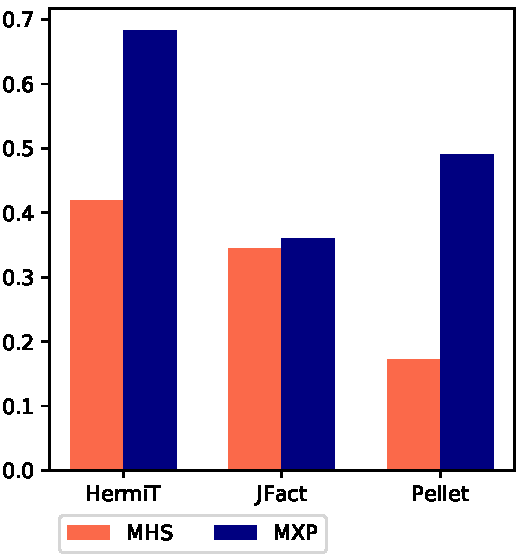
\includegraphics[width=9cm]{eval1Family} 	
	\caption{Family ontology - Experiment 1}
	\label{fig:eval1Family}
\end{figure}

\begin{figure}[H]
	\centering
	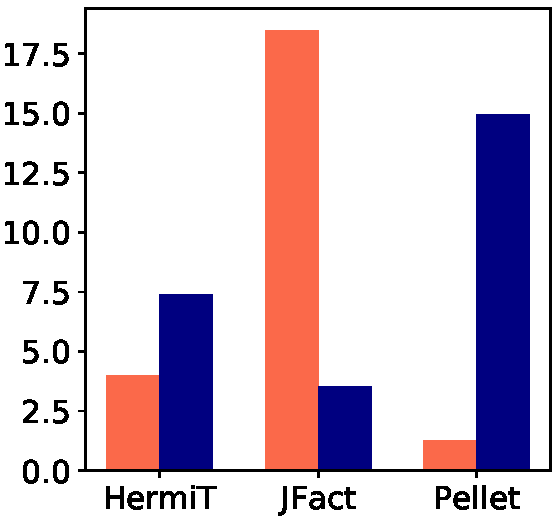
\includegraphics[width=9cm]{eval1Beer} 
	\caption{Beer ontology - Experiment 1}
	\label{fig:eval1Beer}
\end{figure}

\begin{figure}[H]
	\centering
	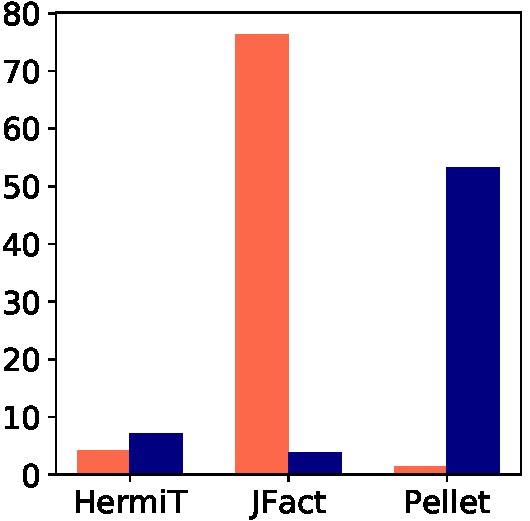
\includegraphics[width=9cm]{eval1LUBM} 
	\caption{LUBM ontology - Experiment 1}
	\label{fig:eval1LUBM}
\end{figure}

\subsection{Experiment 2}

\begin{figure}[H]
	\centering
	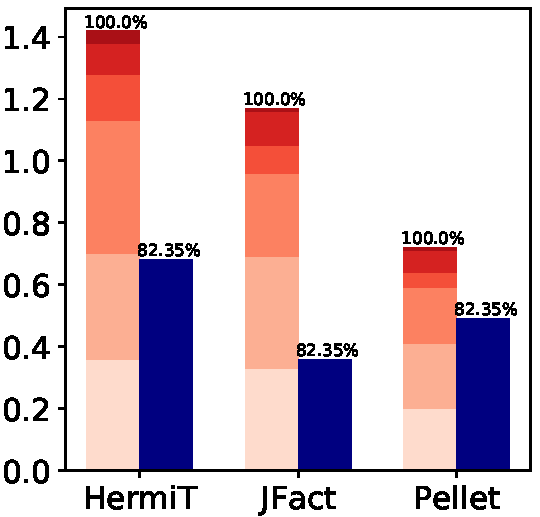
\includegraphics[width=9cm]{eval2Family} 	
	\caption{Family ontology - Experiment 2}
	\label{fig:eval2Family}
\end{figure}

\begin{figure}[H]
	\centering
	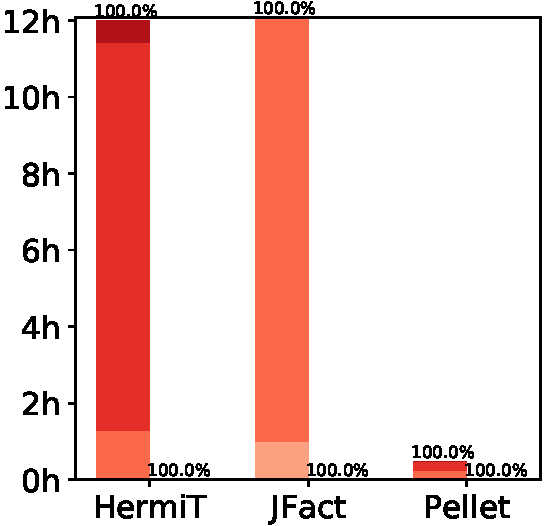
\includegraphics[width=9cm]{eval2Beer} 
	\caption{Beer ontology - Experiment 2}
	\label{fig:eval2Beer}
\end{figure}

\begin{figure}[H]
	\centering
	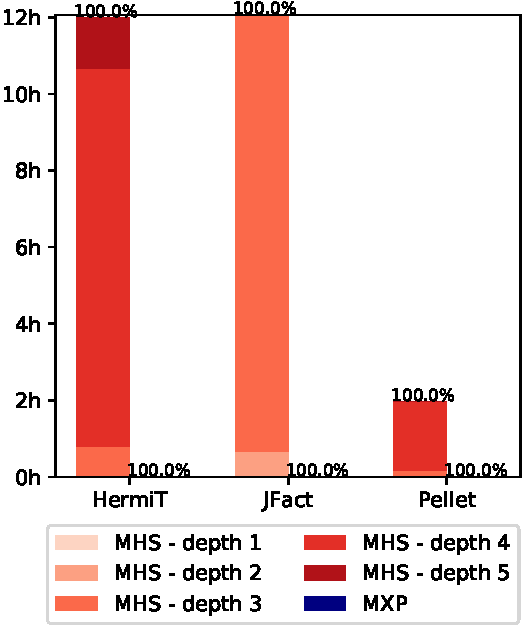
\includegraphics[width=9cm]{eval2LUBM} 
	\caption{LUBM ontology - Experiment 2}
	\label{fig:eval2LUBM}
\end{figure}

\subsection{Conclusion from experiments}


\pagebreak
\section*{Conclusion}
\addcontentsline{toc}{section}{\protect\numberline{}Conclusion}

\pagebreak
\addcontentsline{toc}{section}{\protect\numberline{}References}
\bibliography{references}
\bibliographystyle{unsrtnat}

\pagebreak
\section*{Appendices}
\addcontentsline{toc}{section}{\protect\numberline{}Appendices}

\end{document}